\lab{A Pseudospectral method for periodic functions}{A Pseudospectral method for periodic functions}
\label{lab:pseudospectral2}

\objective{
% We study traveling wave solutions of the Korteweg-de Vries (KdV) equation. 
We look at a pseudospectral method with a Fourier basis, and numerically solve the advection equation using a pseudospectral discretization in space and a Runge-Kutta integration scheme in time.  }

% \section{A Pseudospectral method for periodic functions}
Let $f$ be a periodic function on $[0,2\pi]$. Let $x_1,\ldots,x_N$ be $N$ evenly spaced grid points on $[0,2\pi].$ Since $f$ is periodic on $[0,2\pi]$, we can ignore the grid point $x_0 = 0$. We will further assume that $N$ is even; similar formulas can be derived for $N$ odd. Let $h = 2\pi/N$; then $\{x_1,\ldots,x_N\} = \{h,2h,\ldots,2\pi-h,2\pi\}$.  

The discrete Fourier transform (DFT) of $f$, denoted by $\hat{f}$ or $\mathcal{F}(f)$, is given by
\[
\hat{f}(k) = h \sum_{j=1}^N e^{-ikx_j}f(x_j) \quad \text{ where } k = -N/2+1, \ldots,0,1,\ldots, N/2.
\]
The inverse DFT is then given by
\begin{align}
\begin{split}
f(x_j) &= \frac{1}{2\pi}\sum_{k=-N/2}^{N/2}\frac{e^{ikx_j}}{c_k}\hat{f}(k), \quad j = 1,\ldots, N,
% \\
% &= \frac{1}{2\pi}\sum_{k=-N/2}^{N/2}\!\!{}^{'} e^{ikx_j}\hat{f}(k), \quad j = 1,\ldots, N, 
\end{split}\label{inverse_dft}
\end{align}
where %$\sum_{k=-N/2}^{N/2}\!\!{}^{'}$ is used to denote...
\begin{align}
	c_k = \begin{cases} 2 & \text{if }k = -N/2 \text{ or }k = N/2, \\ 1 &  \text{otherwise.}
\end{cases}
\end{align}
The inverse DFT can then be used to define a natural interpolant (sometimes called a band-limited interpolant) by evaluating (\ref{inverse_dft}) at any $x$ rather than $x_j$:
\begin{align}
p(x) = \frac{1}{2\pi}\sum_{k=-N/2}^{N/2} e^{ikx}\hat{f}(k). \label{interpolant}
\end{align}
The interpolant for $f'$ is then given by 
\begin{align}
p'(x) = ik \frac{1}{2\pi}\sum_{k=-N/2+1}^{N/2-1} e^{ikx}\hat{f}(k). \label{spectral2:deriv}
\end{align}


Consider the function $u(x) = \sin^2 (x) \cos(x) +e^{2\sin(x+1)}$. 
Using \eqref{spectral2:deriv}, the derivative $u'$ may be approximated with the following code.  \footnote{See \textit{Spectral Methods in MATLAB} by Lloyd N. Trefethen.  Another good reference is \textit{Chebyshev and Fourier Spectral Methods} by John P. Boyd.}
We note that although we only approximate $u'$ at the Fourier grid points, \eqref{spectral2:deriv} provides an analytic approximation of $u'$ in the form of a trigonometric polynomial.

\begin{lstlisting}
import numpy as np
from scipy.fftpack import fft, ifft
import matplotlib.pyplot as plt

N=24
x1 = (2.*np.pi/N)*np.arange(1,N+1)
f = np.sin(x1)**2.*np.cos(x1) + np.exp(2.*np.sin(x1+1))


k = np.concatenate(( np.arange(0,N/2) ,
					 np.array([0])	, # Because hat{f}'(k) at k = N/2 is zero.
					 np.arange(-N/2+1,0,1)	))

# Approximates the derivative using the pseudospectral method
f_hat = fft(f)
fp_hat = ((1j*k)*f_hat)
fp = np.real(ifft(fp_hat))

# Calculates the derivative analytically
x2 = np.linspace(0,2*np.pi,200)
derivative = (2.*np.sin(x2)*np.cos(x2)**2. - 
				np.sin(x2)**3. + 
				2*np.cos(x2+1)*np.exp(2*np.sin(x2+1))
				)

plt.plot(x2,derivative,'-k',linewidth=2.)
plt.plot(x1,fp,'*b')
plt.savefig('spectral2_derivative.pdf')
plt.show()

\end{lstlisting}




\begin{figure}
\centering
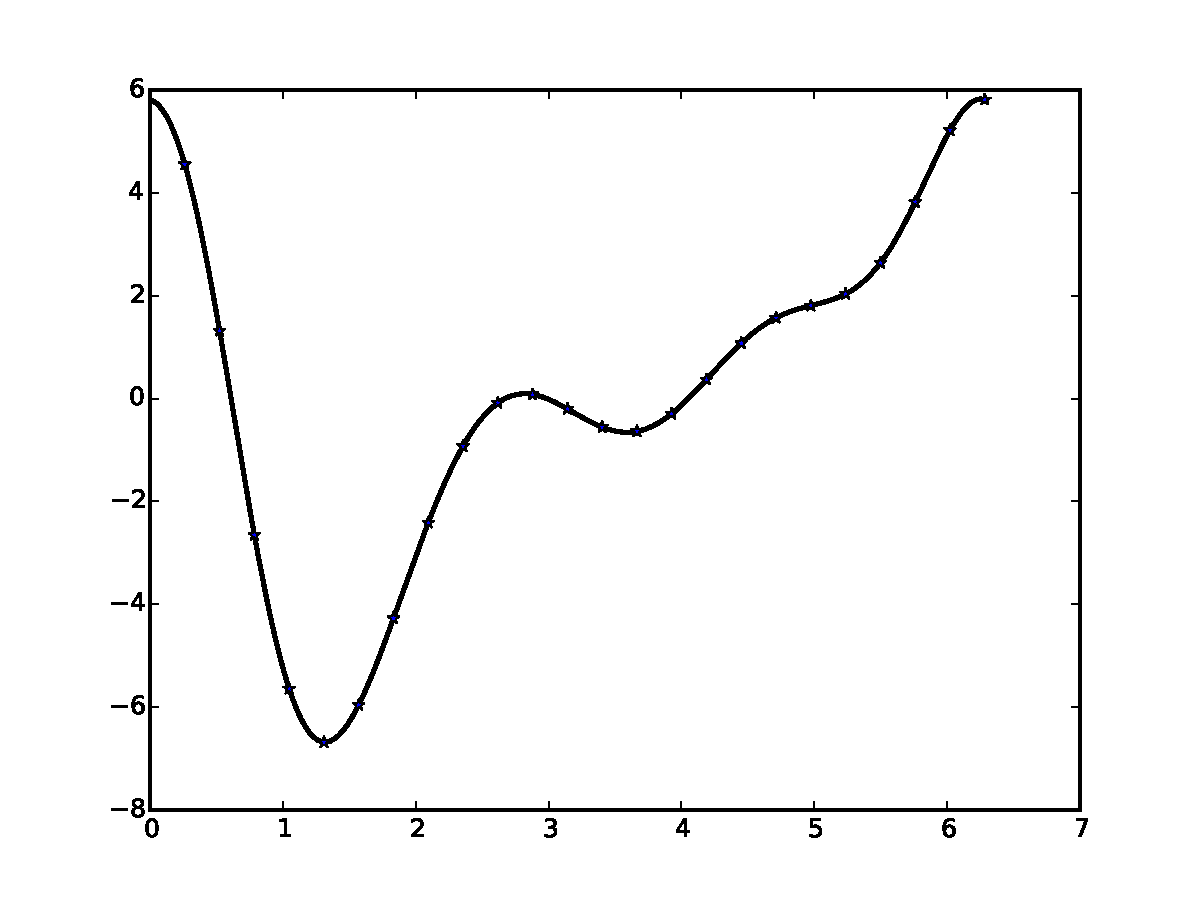
\includegraphics[width=\textwidth]{spectral2_derivative.pdf}
\caption{The derivative of $u(x) = \sin^2 (x) \cos(x) +e^{2\sin(x+1)}$.}
\label{fig:spectral:spectral2_derivative}
\end{figure}

\begin{problem}
Consider again the function $u(x) = \sin^2 (x) \cos(x) +e^{2\sin(x+1)}$.
Create a function that approximates $\frac{1}{2}u''-u'$ on the Fourier grid points for a given $N$.	
\end{problem}

% \begin{lstlisting}
% import numpy as np
% import matplotlib.pyplot as plt
% 
% # Solve the ODE $u_{xx} = e^u,$ with boundary conditions
% #  $u(0) = u(2\pi) = 0$
% 
% 
% \end{lstlisting}


% \begin{problem}
% The motion of a damped pendulum can be described by the ODE
% 	\begin{align}
% 	\theta'' + \theta' +\sin \theta = 0. \label{damped_pendulum}
% 	\end{align}
% Using the pseudospectral method, solve \eqref{damped_pendulum} on the interval $[0,2\pi]$, with the boundary conditions $\theta(0) = \theta(2\pi) =0$. Produce at least two unique solutions.
% \end{problem}

% \section{The KdV equation}
% 
% There are canonical model equations for various types of phenomena.  Long, small amplitude waves moving in one direction can generally be described by the  Korteweg-de Vries (KdV) equation. The KdV equation is given by 
% \[  \frac{\partial u }{\partial t} + u \frac{\partial u}{\partial x} + \frac{\partial^3 u}{\partial x^3} = 0.
% \]
% 
% The KdV equation possesses traveling wave solutions called solitary waves. These traveling waves have the form 
% \[ u(x,t) = 3\alpha^2 \sech^2(\alpha(x-x_0)/2 - \alpha^3 t).
% \]
% 
% History of solitons: first observed by John Scott Russell in 1834. 
% Solution form:  
% Interaction of solitons: 
% 
% Solitons versus solitary waves. I believe solitary waves are solitons in a fluid dynamics context. 
% John Russell 


\section*{The advection equation}
Recall that the advection equation is given by
\begin{align}
&{ }u_t + cu_x = 0
\end{align}
where $c$ is the speed of the wave (the wave travels to the right for $c > 0$).
We will consider the solution of the advection equation on the circle; this essentially amounts to solving the advection equation on $[0,2\pi]$ and assuming periodic boundary conditions. 

A common method for solving time-dependent PDEs is called the \textit{method of lines}. To apply the method of lines to our problem, we use our Fourier grid points in $[0,\pi]$: given an even $N$, let $h = 2\pi/N$, so that $\{x_1,\ldots,x_N\} = \{h,2h,\ldots,2\pi-h,2\pi\}$.  By using these grid points we obtain the collection of equations
\begin{align}
&{ }u_t(x_j,t) + cu_x(x_j,t) = 0, \quad t >0, \quad j = 1, \ldots N. \label{spectral2:method_oflines}
\end{align}

Let $U(t)$ be the vector valued function given by $U(t) = (u(x_j,t))_{j=1}^N$.
Let $\mathcal{F}(U)(t)$ denote the discrete Fourier transform of $u(x,t)$ (in space), so that 
\[
\mathcal{F}(U)(t) = (\hat{u}(k,t))_{k=-N/2+1}^{N/2}.
\]
Define $\mathcal{F}^{-1}$ similarly.
Using the pseudospectral approximation in space leads to the system of ODEs
\begin{align}
	U_t +  \vec{c}\mathcal{F}^{-1}\left(i\vec{k}\mathcal{F}(U) \right) = 0
\end{align}
where $\vec{k}$ is a vector, and $\vec{k}\mathcal{F}(U) $ denotes element-wise multiplication. 
Similarly $\vec{c}$ could also be a vector, if the wave speed $c$ is allowed to vary. 


\begin{problem}
	Using a fourth order Runge-Kutta method (RK4), solve the initial value problem 
	\begin{align}
		u_t +c(x) u_x = 0,
	\end{align}
	where $c(x) = .2 + \sin^2(x-1)$, and $u(x,t=0) = e^{-100(x-1)^2}.$  Plot your numerical solution from $t = 0$ to $t = 8$.  Note that the initial data is nearly zero near $x = 0$ and  $2 \pi$, and so we can use the pseudospectral method. \footnote{This problem is solved in \textit{Spectral Methods in MATLAB} using a leapfrog discretization in time. } 
	\label{spectral2:advection_equation}
\end{problem}



\begin{figure}
\centering
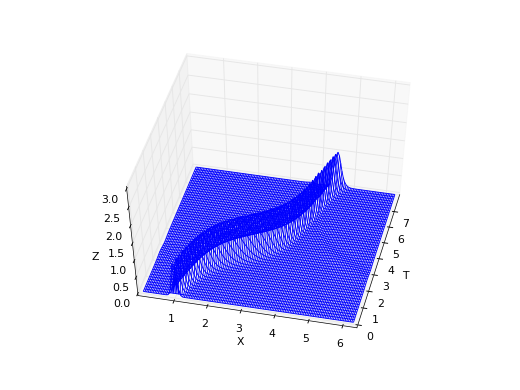
\includegraphics[width=\textwidth]{advection.pdf}
\caption{The solution of the variable speed advection equation; see Problem  \ref{spectral2:advection_equation}.}
\label{fig:spectral:spectral2_advection}
\end{figure}





